\documentclass{article}
\usepackage[utf8]{inputenc}
\usepackage{booktabs}
\usepackage{graphicx}
\usepackage{float}
\usepackage{amsmath}
\usepackage{amssymb}
\usepackage{mathrsfs}
\usepackage{hyperref}
\usepackage[ruled,vlined]{algorithm2e}


\usepackage{lmodern}%
\usepackage{textcomp}%
\usepackage{lastpage}%
\usepackage{longtable}%
\usepackage[a4paper, total={6.3in, 9in}]{geometry}
\usepackage{csquotes}% Recommended
\usepackage{minted}


\begin{document}

\paragraph{Question}
The Pratt \& Whitney Canada PT6 turbo shaft engine is attached to a variable-pitch propeller with a diameter of 1.6m. The engine is operated at 6000ft and Mach 0.3. The pressure ratio of the compressor is 7. Use the below parameters:

\begin{align*}
    \eta_c &= 0.85  &\eta_t &= 0.85 &\eta_m &= 0.9  \\
    \eta_{cc} &= 0.99 & \lambda_cc &= 0.05 &\dot{m} &= 2.75 \text{kg/s}\\
    RR &= 0.99 & \gamma_c &= 1.4 & \gamma_h &= 1.33
\end{align*}
In addition, the temperature at the inlet of the turbine is 1200K and the temperature at the exit of the turbine is 800K. The LHV of the fuel is 43.1 MJ/kg. The efficiencies listed above are \textbf{polytropic}.

\begin{enumerate}
    \item Find the shaft power and residual thrust at the current configuration.
    \item A turboprop engine can be assumed to be constant-speed. If the turbine rotates at a constant speed of 33000 RPM, and the propeller is attached to a gearbox with a gear reduction of 10 and mechanical efficiency of 0.95, find the torque provided to the propeller.
    \item Find the torque, power and power-speed coefficient of the propeller.
    \item Figures \ref{fig:ct} and \ref{fig:cp} shows the power and thrust coefficient at different pitch setting angle against advance ratio. Approximate the pitch setting angle that will balance torque between the propeller and the shaft.
    \item Hence, estimate the total thrust (propeller and residual thrust).
\end{enumerate}

\begin{figure}[H]
    \centering
    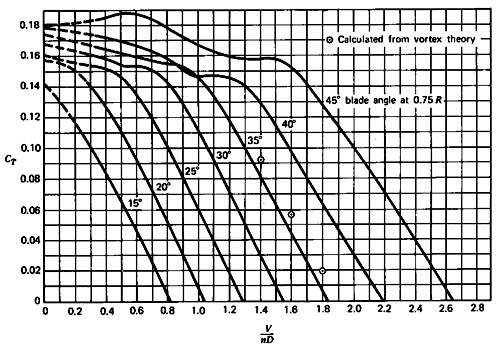
\includegraphics[width=0.8\textwidth]{ct.jpg}
    \caption{Coefficient of thrust versus advance ratio for various pitch settings.}
    \label{fig:ct}
\end{figure}

\begin{figure}[H]
    \centering
    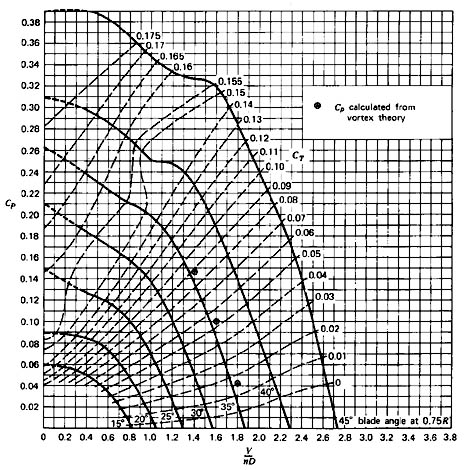
\includegraphics[width=0.8\textwidth]{cp.jpg}
    \caption{Coefficient of power versus advance ratio for various pitch settings.}
    \label{fig:cp}
\end{figure}


\paragraph{Solutions}
I wrote a Python module that makes these calculations much easier. It may be useful for writing these kind of questions in the future. It's very barebone right now but you can check it out on my \href{https://github.com/darentang/pyturb}{GitHub} page.

Ambient Conditions:
\begin{align*}
    T_a &= 276.26 \text{ K}&P_a &= 81.2 \text{ kPa}&V_a &= 99.96 \text{ m/s}
\end{align*}
\begin{enumerate}
    \item \begin{description}
        \item[Station 0]
        \begin{align*}
            T_{t0} &= 276.26(1 + 0.2\times 0.3^2) = 281.27 \text{ K}\\
            P_{t0} &= 81.2(1 + 0.2\times 0.3^2)^{1.4/0.4} = 86.47 \text{ kPa}
        \end{align*}
        \item[Station 2]
        \begin{align*}
            T_{t2} &= T_{t0} = 281.27 \text{ K} \\
            P_{t2} &= RR \cdot P_{t0} = 85.60 \text{ kPa}
        \end{align*}
        \item[Station 3]
        \begin{align*}
            P_{t3} &= \pi_c \cdot P_{t2} = 599.21 \text{ kPa}\\
            T_{t3} &= T_{t2}\pi_c^{\frac{\gamma_c - 1}{\eta \gamma}} = 541.0 \text{ K}
        \end{align*}
        \item[Station 4]
        \begin{align*}
            P_{t4} &= P_{t3}(1-\lambda_{cc}) = 569.25 \text{ kPa}\\
            T_{t4} & = TIT = 1200 \text{ K}
        \end{align*}
        \item[Combustion Chamber]
        \begin{align*}
            FAR &= \dfrac{1156.7(1200-288) - 1004.5(541.0 - 288)}{0.99\times 43.1\times 10^6 - 1156.7(1200 - 288)}\\
            &= 0.01924
        \end{align*}

        \item[Turbine Compressor Balance]
        \begin{align*}
            P_{comp} &= \dot{m} c_{p, c} (T_{t3} - T_{t2}) \\
            &=2.75\cdot 1004.5 \cdot(541 - 281.27) \\ 
            &=717.472 \text{ kW}\\
            P_{turb} &= \dot{m} (1 + FAR) c_{p, h} (T_{t4} - T_{t5}) \\
            &=2.75\cdot 1.01924\cdot 1156.7 \cdot(1200 - 800) \\ 
            &=1296.850 \text{ kW}\\
            P_{offtake} &= \eta_m P_{turb} - P_{comp} = 449.725 \text{ kW}
        \end{align*}
    
        \item[Station 5]
        \begin{align*}
            P_{t5} &= 569.25 \cdot \dfrac{800}{1200}^{\frac{1.33}{0.33\dot 0.85}}\\
            &= 83.25 \text{ kPa}
        \end{align*}

        \item[Station 9]
        \begin{align*}
            T_{t9} &= T_{t5} = 800\text{ K}\\
            NPR &= \frac{P_{t9}}{P_a} = 1.025 \\
            \pi_{crit} &= (1 + (\gamma_h - 1 )/2)^\frac{\gamma_h}{\gamma_h - 1} = 1.85
        \end{align*}
        $NPR < \pi_{crit}$. The nozzle is adapted.
        \begin{align*}
            P_9 &= P_a = 81.23 \text{ kPa}\\
            T_9 &= T_{t5}\cdot \frac{1}{NPR}^\frac{\gamma_h - 1}{\gamma_h} = 795.16 \text{ K} \\
            M_9 &= \sqrt{\frac{2}{\gamma_h - 1} \left( NPR ^\frac{\gamma_h - 1}{\gamma_h} - 1\right)} = 0.192 \\
            V_9 &= M_9 \sqrt{\gamma R T} = 105.86 \text{ m/s}\\
            A_9 &= \frac{\dot{m}}{\rho V} = 0.073 \text{ m}^2
        \end{align*}
        \item[Residual Thrust]
        \begin{align*}
            T_{res} = F_{net} = \dot{m}(1 + FAR)V_9 - \dot{m}V_a + (P_9 - P_a)A_9 = 21.85 \text{ N}
        \end{align*}
    \end{description}
    \item The turbine rotates at 33000 RPM, which is 550 revolutions per second. The gear has a reduction of 10 so the propeller rotates 55 revolutions per second. Therefore:
    \begin{align*}
        Q &= \dfrac{\eta_{gear} P_{shaft}}{\Omega_{shaft}}\\
        &= \dfrac{0.95 \cdot 449.725\times 10^3 }{55 \times 2\pi} \\
        &= 1236.31 \text{ Nm}
    \end{align*}

    \item The torque, power and power-speed coefficients are:
    \begin{align*}
        C_Q &= \dfrac{Q}{\rho n_{prop}^2 D^5} = 0.0466 \\ 
        C_P &= 2 \pi C_Q = 0.293 \\ 
        C_S &= \left(\dfrac{\rho V_a^5}{P n_{prop}^2}\right)^{1/5} = 8.057
    \end{align*}

    \item The advance ratio is:
    \begin{align*}
        J &= \dfrac{V_a}{n_{prop}D} = 1.136
    \end{align*}
    Figure \ref{fig:cp_interp} shows the interpolated values based on Figure \ref{fig:cp}. The red start marks the point of (1.136, 0.293). The interpolated value for $\beta$ is $42.5^\circ$. 

    \begin{figure}[H]
        \centering
        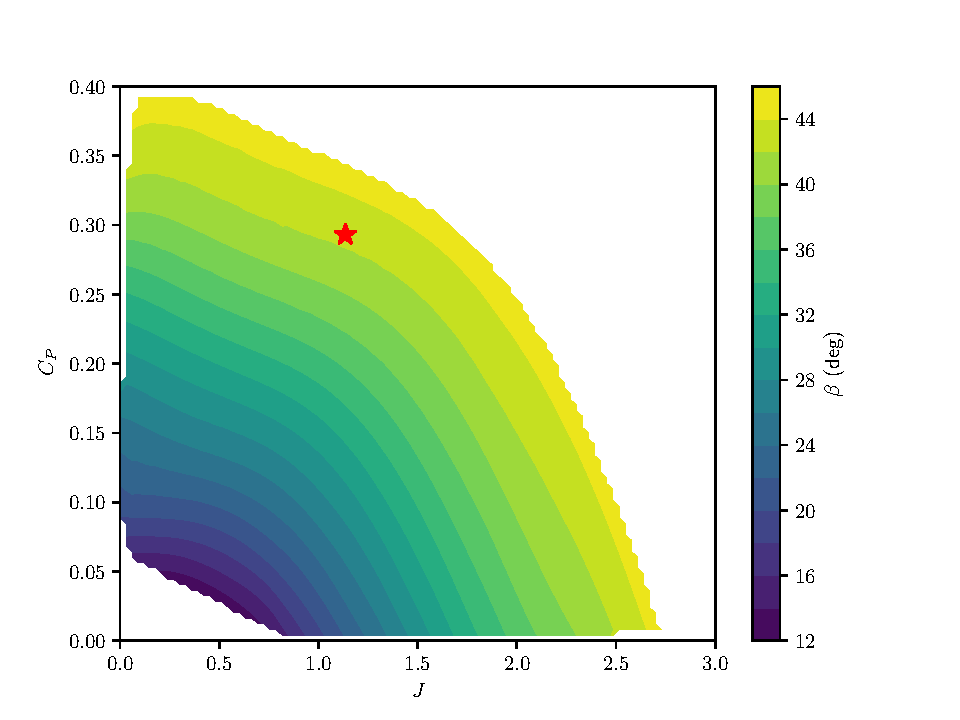
\includegraphics[width=0.8\textwidth]{cp_interp.pdf}
        \caption{Interpolated values for $C_P$.}
        \label{fig:cp_interp}
    \end{figure}

    \item Based on Figure \ref{fig:ct}, the coefficient of thrust at $J = 1.136$ and $\beta = 42.5^\circ$ is approximately 0.15. Therefore the thrust provided by the propeller is:
    \begin{align*}
        T_{prop} = C_T \rho n_{prop}^2 D^4 = 2486.31\text{ N}
    \end{align*}
    Therefore, the total thrust (including residual thrust) is:
    \begin{align*}
        T_{total} = T_{prop} + T_{net} = 2508.16
    \end{align*}
    Appropriate comments about how much the residual thrust contributes to the total thrust should also be considered.
\end{enumerate}

\end{document}